\section{Gestão de Tempo}
Cada \gls{sprint} do projeto terá a duração de 2 semanas (10 dias úteis) e respeitará
todas as cerimônias do \gls{scrum}. Antes de dar início a uma nova sprint
ocorrerá a realização da \gls{planning}, reunião de planejamento onde
serão definidos os entregáveis da Sprint a ser iniciada. Após o início
da iteração, as dailies serão feitas através do grupo de mensagens
instantâneas do time. Ao fim do período de 2 semanas, ocorrerá a
\gls{review}, reunião com o objetivo de avaliar o que foi entregue
com sucesso naquela Sprint, e também a \gls{retrospective}, reunião
onde a equipe conversa sobre os pontos positivos e negativos da última
iteração e o que pode ser melhorado para a próxima Sprint. Todas essas
cerimônias foram incluídas no planejamento de gestão de tempo para o
cálculo da quantidade de Sprints necessárias até a entrega final do
projeto.

\begin{figure}[H]
  \centering
  \caption{Timeline do projeto}
  \label{fig:cli-srv}
  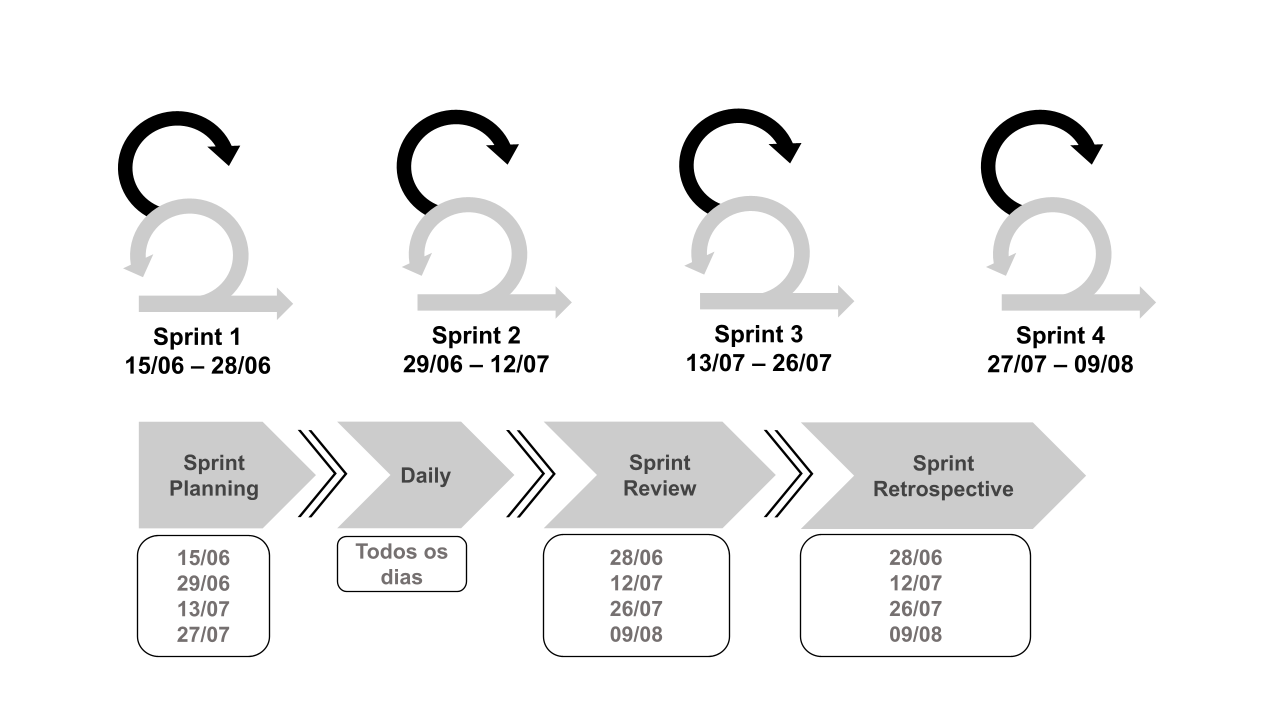
\includegraphics[scale=0.3]{Timeline}
	\fonte{Os Autores}
\end{figure}

%%% Local Variables:
%%% mode: latex
%%% TeX-master: "../../desenho"
%%% End:
